\chapter{Unit Tests}
\section{10 Unit Tests}
Tabelle irgendwo in diesem Kapitel. Latex packt die dahin wo es das für richtig hält
\afterpage{%
	\clearpage% Flush earlier floats (otherwise order might not be correct)
	\thispagestyle{empty}% empty page style (?)
	\begin{landscape}% Landscape page
		\centering % Center table
		\begin{adjustbox}{center,caption={Evaluation der Datensätze},float=table,label={tab:Datasets}}
			\centering
			\label{tab:Datasets}
			\small
			\setlength{\tabcolsep}{3pt}
	\begin{tabular}{l|l}
		Unit Test                                & Beschreibung                                                                       \\ \hline
		RPGCharacterTest\#getAC()                & Es wird geprüft ob die Armor Class (AC) des Charackters korrekt berechnet wird.    \\ \hline
		RPGCharacterTest\#getSavingThrows()      & Es wird geprüft ob die SavingThrows Boni des Charackters korrekt berechnet werden. \\ \hline
		RPGCharacterTest\#getSkills()            & Es wird geprüft ob die Skill Boni des Charackters korrekt berechnet werden.        \\ \hline
		DeathSavesTest\#getFailures()            & Prüft ob die Anzahl an Fehlschlägen korrekt berechnet wird.                        \\ \hline
		DeathSavesTest\#getSuccesses()           & Prüft ob die Anzahl an Erfolgreichen Death Saves korrekt berechnet wird            \\ \hline
		DiceRollServiceTest\#rollInitiative()    & Prüft ob das Ergebnis des Initiative Wurfs korrekt berechnet wird                  \\ \hline
		DiceRollServiceTest\#attack()            & Prüft ob der Damage beim Ausführen einer Attacke korrekt berechnet wird            \\ \hline
		DiceRollServiceTest\#rollSkill()         & Prüft ob das Ergebnis eines Skill Rolls korrekt berechnet wird                     \\ \hline
		DiceRollServicetest\#rollSavingThrow()   & Prüft ob das Ergebnis eines SavingThrows korrekt berechnet wird                    \\ \hline
		CharacterServiceTest\#displayCharacter() & Prüft ob der String eines Charackters korrekt zusammengebaut wird.                
	\end{tabular}
       % \caption{Evaluation der Datensätze}
\end{adjustbox}
% Add 'table' caption
\end{landscape}
\clearpage% Flush page
}
\section{ATRIP: Automatic}
Automatic wurde auf zwei verschiedene Arten und weisen realisiert, einmal wurde die pom.xml des Maven Projektes im Hauptmodul der Applikation so angepasst, das das automatische Ausführen aller Tests Teil des Maven Workflows ist. Somit werden Tests automatisch mit jedem maven package, test und install ausgeführt. Sollte ein Test fehlschlagen, wird der jeweilige maven Workflow nicht erfolgreich abgeschlossen. Desweiteren wurde ein Github workflow zur automatischen Validierung aller Pullrequests und Commits angelegt. Dieser Workflow führt nach jedem Commit in einer isolierten Umgebung den maven package workflow aus. Kommt es während dieses zu einem Test Failure, schlägt der Workflow fehl und die Pullrequest kann nicht gemerged werden, oder es wird explizit am Commit ausgewiesen, dass dieser Commit fehlerhaft ist.

\clearpage
\section{ATRIP: Thorough}
\lstinputlisting[
label={code:diceRollThorough},  % Label; genutzt für Referenzen auf dieses Code-Beispiel
caption={Test der Attack Methode des DiceRollService},
captionpos=b,               % Position, für die Caption:  t(op) oder b(ottom)
language=java,     % Eigener Style der vor dem Dokument festgelegt wurde
firstline=36,                % Zeilennummer im Dokument welche als erste angezeigt wird
lastline=51,                 % Letzte Zeile welche ins LaTeX Dokument übernommen wird
basicstyle=\tiny
]{Quellcode/DiceRollServiceTest.java}
In Listing \ref{code:diceRollThorough}, ist ein Beispiel zu sehen, bei dem alle notwendigen Funktionalitäten der \texttt{attack()} Methode getestet werden. So testet der Unit Test das korrekte berechnen von Werten unter Einbezug aller möglicher Eigenschaften einer Waffe, sowie das auftreten von Exception, in dem absichtlich falsche Eingaben an die Funktion gereicht werden. Somit dekt dieser Test alle Funktionalitäten der Methode vollständig ab und hält damit das Thorough Prinzip ein. Im Vergleich dazu,hält der in Listing \ref{code:diceRollNotThorough} gezeigte Test dieses Prinzip nicht ein. Er überprüft nur eine mögliche valide Eingabe und prüft keine Randfälle und falsch Eingaben. Somit wird nicht kontrolliert, ob nach veränderungen Exceptions noch korrekt geworfen werden oder ob ungewollte Seiteneffekte auftreten. 
\lstinputlisting[
label={code:diceRollNotThorough},  % Label; genutzt für Referenzen auf dieses Code-Beispiel
caption={Test der rollSkill Methode des DiceRollService},
captionpos=b,               % Position, für die Caption:  t(op) oder b(ottom)
language=java,     % Eigener Style der vor dem Dokument festgelegt wurde
firstline=53,                % Zeilennummer im Dokument welche als erste angezeigt wird
lastline=56,                 % Letzte Zeile welche ins LaTeX Dokument übernommen wird
basicstyle=\tiny
]{Quellcode/DiceRollServiceTest.java}

\section{ATRIP: Professional}
\lstinputlisting[
label={code:diceRollProfessional},  % Label; genutzt für Referenzen auf dieses Code-Beispiel
caption={Auszug aus dem Test des DiceRollService, ganzes File: \href{https://github.com/lkno0705/DnD-CharacterManager/blob/main/2-dnd-charactermanager-application/src/test/java/rolls/DiceRollServiceTest.java}{https://github.com/lkno0705/DnD-CharacterManager/blob/main/2-dnd-charactermanager-application/src/test/java/rolls/DiceRollServiceTest.java}},
captionpos=b,               % Position, für die Caption:  t(op) oder b(ottom)
language=java,     % Eigener Style der vor dem Dokument festgelegt wurde
firstline=63,                % Zeilennummer im Dokument welche als erste angezeigt wird
lastline=97,                 % Letzte Zeile welche ins LaTeX Dokument übernommen wird
basicstyle=\tiny
]{Quellcode/DiceRollServiceTest.java}
Listing \ref{code:diceRollProfessional} zeigt ein positives Beispiel des Professional Prinzips. In diesem Beispiel wurde Test Code wie Produktivcode behandelt und es wurde darauf geachtet, den Prozess des Mockings anstatt in einer riesigen Methode in mehrere kleine Untermethoden zu unterteilen. Somit ist der Code gut wartbar und falls eine Änderung gemacht werden muss, kann man sofort zu der jeweiligen Methode springen und muss nicht in einer Wall of Text die entsprechende Stelle raussuchen. Des weiteren kümmert sich jede Methode in diesem Beispiel genau um eine einzige Funktionalität. Somit wird in jeder Methode nur genau ein Mockobjekt generiert.
\lstinputlisting[
label={code:diceRollNotProfessional},  % Label; genutzt für Referenzen auf dieses Code-Beispiel
caption={Auszug aus dem Test des DiceRollService, ganzes File: \href{https://github.com/lkno0705/DnD-CharacterManager/blob/main/2-dnd-charactermanager-application/src/test/java/character/CharacterServiceTest.java}{https://github.com/lkno0705/DnD-CharacterManager/blob/main/2-dnd-charactermanager-application/src/test/java/character/CharacterServiceTest.java}},
captionpos=b,               % Position, für die Caption:  t(op) oder b(ottom)
language=java,     % Eigener Style der vor dem Dokument festgelegt wurde
firstline=118,                % Zeilennummer im Dokument welche als erste angezeigt wird
lastline=136,                 % Letzte Zeile welche ins LaTeX Dokument übernommen wird
basicstyle=\tiny
]{Quellcode/CharacterServiceTest.java}
Wie in Listing \ref{code:diceRollNotProfessional} kommt das Mocking von \texttt{HitDice}, \texttt{Weapons} etc. in anderen Tests auch zum Einsatz. Trotz dessen das auch in diesen Tests darauf geachtet wurde, den Mocking Prozess in kleine Methoden aufzuspalten und somit die Wartbarkeit und lesbarkeit zu erhöhen, stellt dies doch auch gleichzeitig ein negativ Beispiel dar. Da nun in jedem Test der ein Entsprechendes Objekt mockt, eine Änderung gemacht werden muss, wenn etwas an den jeweiligen Domain Objekten geändert wurde. Somit währe es hier sinnvoll gewesen, den Mocking Prozess in eine Utility Class auszulagern. Dies würde nicht nur die Wartbarkeit und lesbarkeit des Tests verbessern, sondern auch gleichzeitig die komplexität der Tests verringern.

\section{Code Coverage}
\begin{figure}[H]
	\centering
	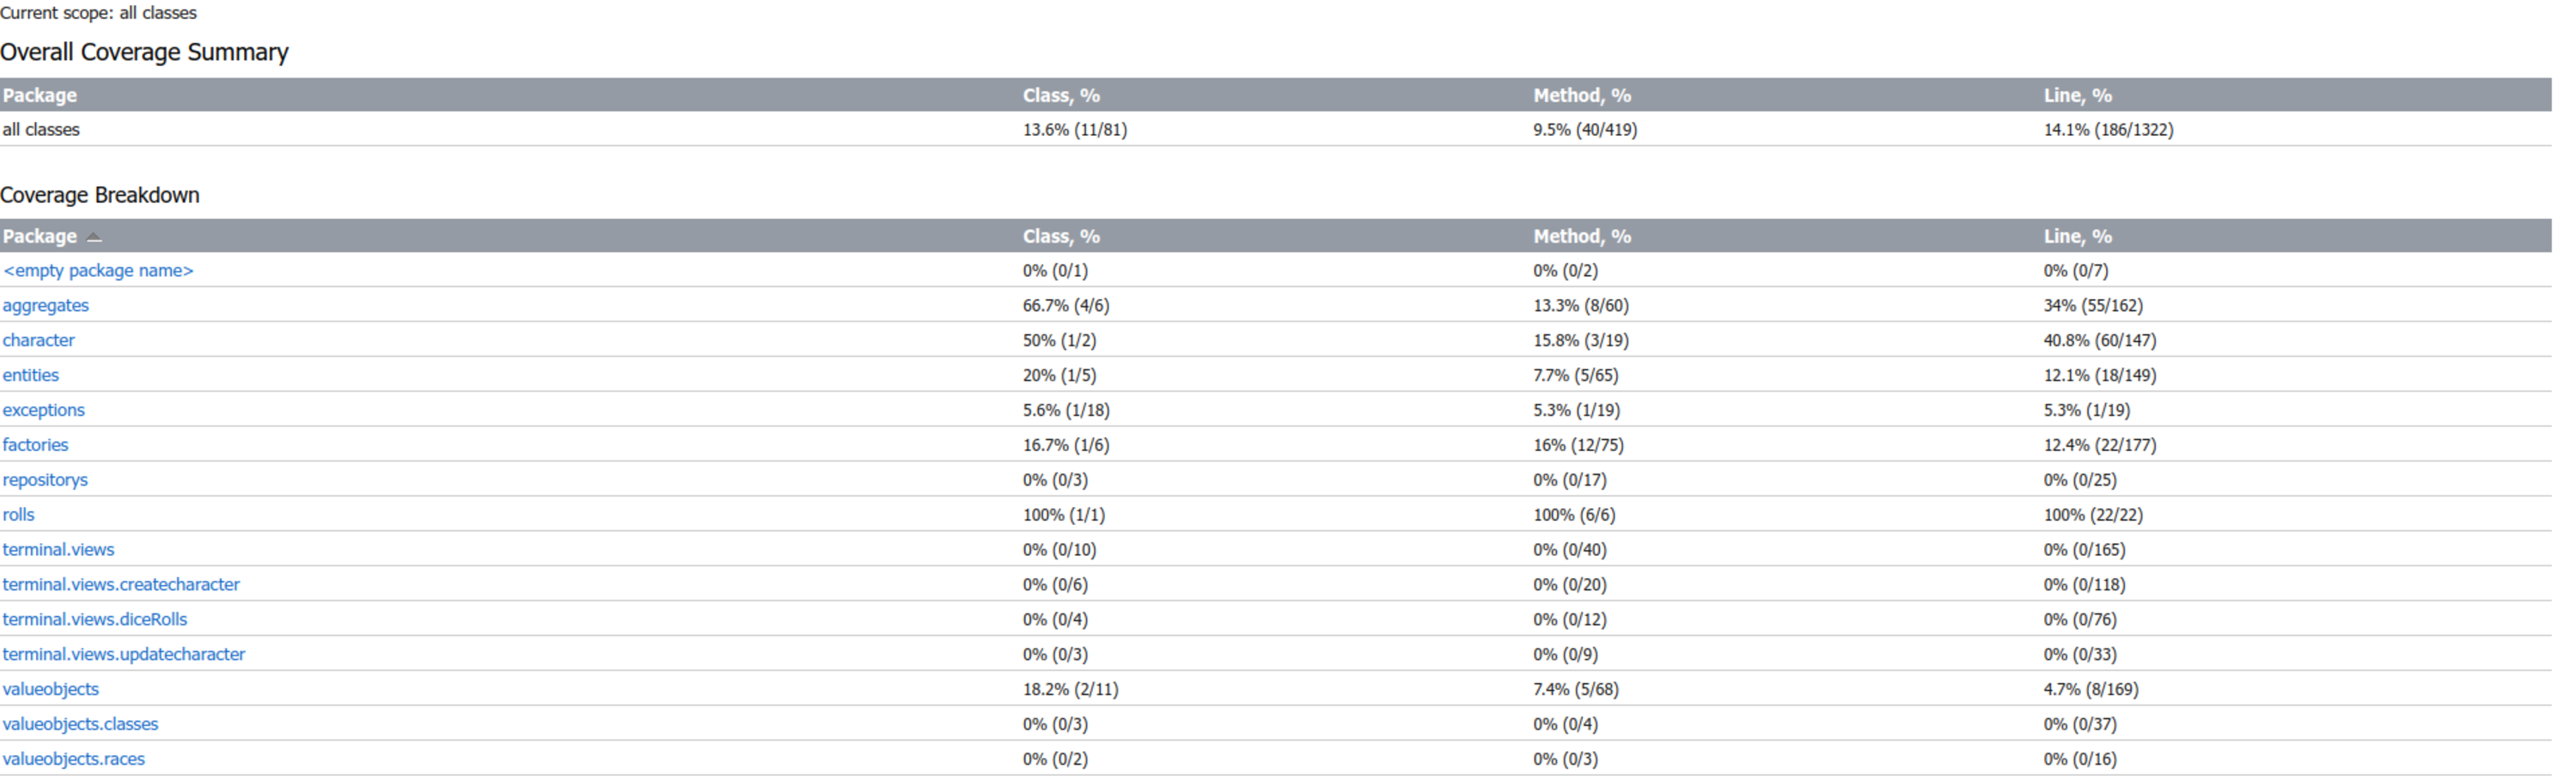
\includegraphics[width=\textwidth]{Bilder/CodeCoverage.pdf}
	\caption{Code Coverage Report generiert von IntelliJ}
	\label{fig:CodeCoverage}
\end{figure}
Abbildung \ref{fig:CodeCoverage} zeigt den Code Coverage report der Tests über das gesamte Projekt. Die generelle Coverage ist mit einer Line Coverage von 14.1\%, einer Class Coverage von 13.6\% und einer Method Coverage von 9.5\% recht gering. Dies liegt daran das der größte Teil des Projektes ausschließlich aus der Modellierung von Domänenobjekten besteht, die ausschließlich Setter und Getter enthalten und nicht sehr viel Logik mit sich bringen. Diese Objekte werden in den jeweiligen Unit Tests durch mocks ersetzt und somit nicht durchlaufen. Daher entstehen sehr geringe Coverage Prozent zahlen. In Packages wie dem \texttt{rolls} Package ist das anders. Dieses Package enthält die UseCases des \texttt{DiceRollService}, die jeweils für den Nutzer wichtige Ergebnisse berechnen. Diese lassen sich sinnvoll und gut testen. Somit erreicht die Code Coverage in diesem Package auch einen Wert von 100\% in allen 3 Coverage Kategorien. Um die Code Coverage zu verbessern wären in diesem Projekt Integration Tests sinnvoll. Da sie neben der reinen Funktionalität einzelner Methoden, auch das zusammenspiel der einzelnen Klassen und Objekte prüfen und somit auch prüfen können ob Dinge richtig gesetzt und gelesen werden und ob die Semantik der Prozesse korrekt ist.

\section{Fakes und Mocks}
\begin{figure}[H]
	\centering
	\includegraphics[width=\textwidth]{Bilder/CharacterServiceTest.pdf}
	\caption{Abhängigkeiten der CharacterService Klasse}
	\label{fig:Mocks}
\end{figure}
Wie Abbildung \ref{fig:Mocks} zu entnehmen ist, hängt die Klasse \texttt{CharacterService} von allen Klassen der Domain Schicht ab und hat somit sehr viele Abhängigkeiten. Ein Unit Test soll jedoch möglichst wenige bis gar keine Abhängigkeiten besitzen, um den Test und die auftretenden Effekte auf einen Ort zu isolieren und zu beschränken. Um dies zu ermöglichen und die Abhängigkeiten der Klassen zu reduzieren, wurde jedes einzelne Objekt, von dem der \texttt{CharacterService} abhängig ist durch einen Mock / einen Fake ersetzt. Dementsprechend wurden folgende Klassen ersetzt:
\begin{itemize}
	\item \texttt{HitDie}
	\item \texttt{Weapon}
	\item \texttt{RepositoryService}
	\item \texttt{Player}
	\item \texttt{CharacterClass}
	\item \texttt{Personality}
	\item \texttt{Background}
	\item \texttt{CharacterRace}
	\item \texttt{DeathSaves}
	\item \texttt{Attributes}
	\item \texttt{Currencys}
	\item \texttt{Armor}
	\item \texttt{Inventory}
	\item \texttt{RPGCharacter}
\end{itemize}
Wären diese Objekte nicht durch Fakes ersetzt worden, hätte dieser Test praktisch das gesamte Projekt getestet. Ein ähnlicher Fall stellt auch der \texttt{DiceRollServiceTest} dar, auch wenn dieser weniger Abhängigkeiten besitzt.